\chapter{Introduction to LBNF and DUNE}
\label{ch:physics-intro}


%\section{chd:physics-intro-overview}
% This text taken from Volume 1, section 1.1

The \dword{dune} will be a world-class neutrino observatory and nucleon decay detector designed to answer fundamental questions about elementary particles and their role in the universe. The international \dword{dune} experiment, hosted by the U.S. Department of Energy's \dword{fnal}{}, will consist of a \dword{fd} located about \SI{1.5}{km} underground at the \dword{surf} in South Dakota, USA, \SI{1300}{\km} from \dword{fnal}{}, and a \dword{nd} located on site at \dword{fnal} in Illinois. The far detector will be a very large, modular \dword{lartpc} with a total mass of nearly \SI{70}{kt} of \dword{lar}, at least \fdfiducialmass (\SI{40}{\giga\gram}) of which is fiducial. The \dword{lar} technology 
has the unique capability to reconstruct neutrino interactions with image-like precision and unprecedented resolution. 

The \dword{dune} detectors will be exposed to the world's most intense neutrino beam originating at \dword{fnal}{}. A high-precision near detector, \SI{574}{m} from the neutrino source on the \dword{fnal} site, will be used to characterize the intensity and energy spectrum of this wide-band beam. The ability to compare the energy spectrum of the neutrino beam between the \dword{nd} and \dword{fd}
is crucial for discovering new phenomena in neutrino oscillations. The \dword{lbnf}, also hosted by \dword{fnal}, provides the infrastructure for this complex system of detectors at the Illinois and South Dakota sites. \dword{lbnf} is responsible for the neutrino beam, the deep-underground site, and the infrastructure for the \dword{dune} detectors. 

%%%%%%%%%%%%%%%%%%%%%%%%%%%%%%%%%%%%%%%%%%%%%%%%%%%%%%%%%%%%%%%%
% This section taken from Volume 1, section 1.3
\section{The LBNF Facility}
\label{sec:physics-intro-lbnf}

The \dword{lbnf} project is building the facility that will house and provide infrastructure for the first two \dword{dune} \dword{fd} modules  in South Dakota  and the \dword{nd} in Illinois.  Figure~\ref{fig:lbnf} shows
a schematic of the facilities at the two sites, and Figure~\ref{fig:caverns} shows a diagram of the cavern layout for the \dword{fd}.  
The organization and management of \dword{lbnf} is separate from the \dword{dune} collaboration. \dword{lbnf} is also hosted by \dword{fnal} and its design and construction are organized as a \dword{doe}/\dword{fnal} project incorporating international partners. 

\begin{dunefigure}[ 	
LBNF/DUNE project: beam from Illinois to South Dakota]{fig:lbnf}{ 	
LBNF/DUNE project: beam from Illinois to South Dakota.}
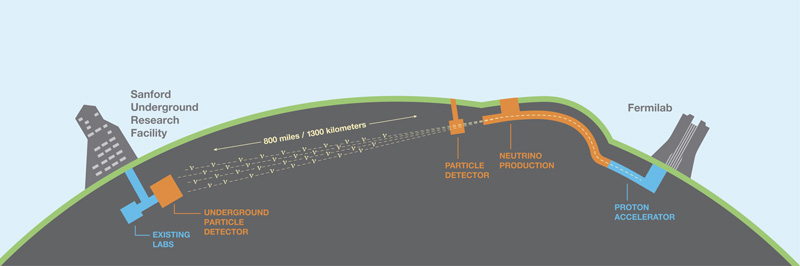
\includegraphics[width=0.9\textwidth]{lbnf_dune_graphic_miles_km-15-0031-01.jpg}
%\label{fig:mhexec}
\end{dunefigure}

\begin{dunefigure}[ 	
Underground caverns for DUNE in South Dakota]{fig:caverns}{Underground caverns for DUNE FD and cryogenics systems at \dword{surf}, in South Dakota. The drawing, which looks towards the northeast, shows the first two far detector modules in place.}
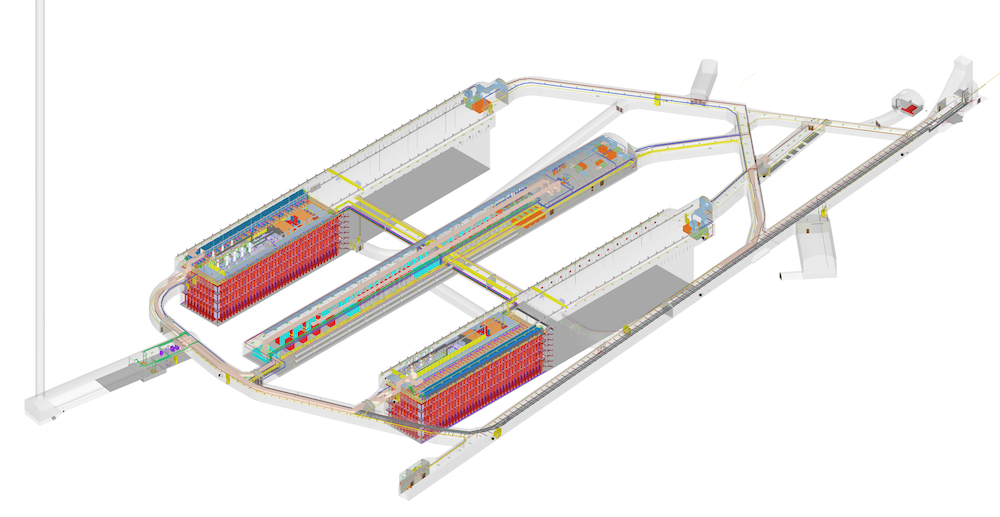
\includegraphics[width=0.99\textwidth]{caverns_full_assembly}
\end{dunefigure}


%Specifically, \dword{lbnf} provides
The \dword{lbnf} project provides to \dword{dune}
\begin{itemize}
\item  the  technical and conventional facilities for a powerful neutrino beam utilizing the \dword{pip2} upgrade~\cite{pip2-2013} of the \dword{fnal} accelerator 
complex. The \dword{pip2} project will deliver between \SIrange{1.0}{1.2}{MW} of proton beam power from \dword{fnal}'s Main Injector in the energy range  \SIrange{60}{120}{GeV} at the start of \dword{dune} operations and provide a platform for extending beam power to \dword{dune} to %multi-MW capability (
$>\,$\SI{2}{MW}. %). 
A further planned upgrade 
of the accelerator complex will enable it to provide up to \SI{2.4}{\MW} of beam power by 2030. 

\item  the civil construction, or \dword{cf}, for the \dword{nd} systems at \dword{fnal}; (see Figure~\ref{fig:beamline});

\item the excavation of three underground caverns at \dword{surf} to house the \dword{dune} \dword{fd}. The north and south caverns will each house two cryostats with 
a minimum \nominalmodsize fiducial mass of liquid argon, while the \dword{cuc} will house cryogenics and data acquisition facilities for all four detector modules;

\item surface, shaft, and underground infrastructure to support 
the outfitting of the caverns with four free-standing, steel-supported cryostats 
and the required cryogenics systems to enable rapid deployment of the first two \nominalmodsize \dword{fd} modules. 
The intention is to install the third and fourth cryostats as rapidly as funding will 
allow.

\end{itemize}


\begin{dunefigure}[Neutrino beamline and DUNE near detector hall in Illinois
]{fig:beamline}{Neutrino beamline and DUNE near detector hall at Fermilab in Illinois}
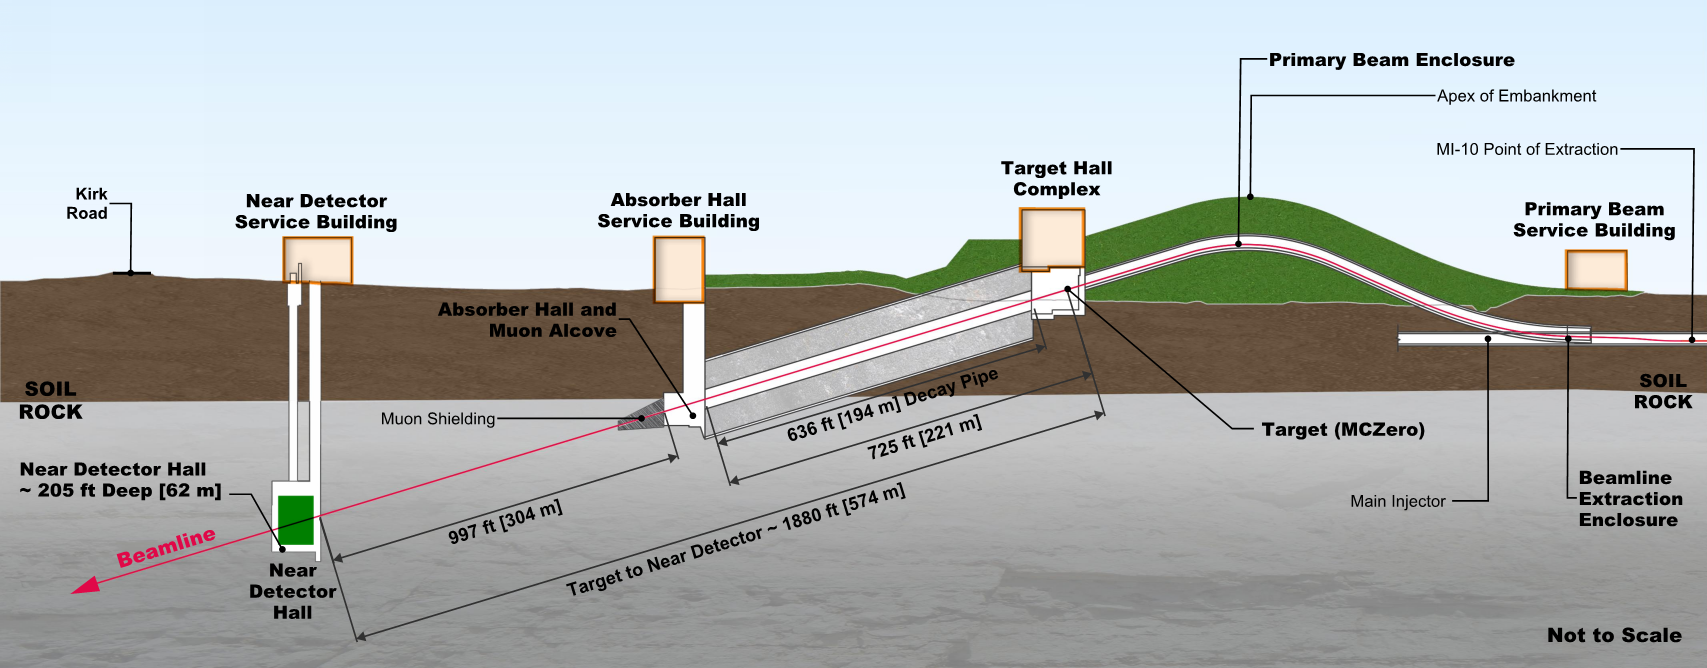
\includegraphics[width=0.95\textwidth]{beamline-sideview.jpg}
\end{dunefigure}

%%%%%%%%%%%%%%%%%%%%%%%%%%%%%%%%%%%%%%%%%%%%%%%%%%%%%%%%%%%%%%%%
% This section taken from Volume 1, section 1.4
\section{\dshort{dune}: Far Detector Modules}
\label{sec:physics-intro-dunefd}

The %\fdfiducialmass 
\dword{dune} \dword{fd} consists of four \dword{lartpc} \dwords{detmodule}, each contained in a cryostat that holds \larmass of \dword{lar}. Each module, installed approximately \SI{1.5}{km} underground, has a fiducial mass of at least \nominalmodsize. The \dword{lartpc} technology provides
excellent tracking and calorimetry performance, making it an ideal
choice for the \dword{dune} \dword{fd}. Each of the \dwords{lartpc} fits inside a cryostat of internal dimensions
\cryostatwdth (W) $\times$ \cryostatht (H) $\times$ \cryostatlen~(L) that contains a total \dword{lar} mass of about \larmass{}.
 The four identically sized modules provide flexibility for staging construction and for evolution of \dword{lartpc} technology.

\dword{dune} is planning for and is prototyping two \dword{lartpc} technologies:
\begin{itemize}
\item \Dword{sp}: In the \dword{sp} technology, ionization charges are drifted horizontally in \dword{lar} and read out on wires in the liquid.  The maximum drift length in the first \dword{dune} \dword{spmod} is \spmaxdrift, and the nominal drift field is \spmaxfield, corresponding to a cathode \dword{hv} of \sptargetdriftvoltpos. This design requires very low-noise electronics to achieve readout with good \dword{s/n} because no signal amplification occurs in the liquid. This technology was pioneered by the \dword{icarus} project, and after several decades of worldwide R\&D, is now a mature technology. It is the technology used for \dword{fnal}'s currently operating \dword{microboone} detector, as well as the \dword{sbnd} detector, which is under construction. 

\item \Dword{dp}: This technology was pioneered at a large scale by the \dword{wa105} collaboration at \dword{cern}. It is less established than the \dword{sp} technology but offers a number of potential advantages. Here, ionization charges drift vertically in \dword{lar} and are transferred into a layer of gas above the liquid. Devices called \dwords{lem} amplify the signal charges  in the gas phase. The gain achieved in the gas reduces stringent requirements on the electronics, and increases the possible drift length, which, in turn, requires a correspondingly higher voltage. The nominal drift field is \dpnominaldriftfield, as for the \dword{sp} detector, but in this case corresponds to a cathode \dword{hv} of \dptargetdriftvoltpos.
The maximum drift length in the \dword{dpmod} is \dpmaxdrift{}.  
\end{itemize}
%from Justin's SP exec summ
In both technologies, the drift volumes are surrounded by a \dword{fc} that defines the volume(s) and ensures uniformity of the \efield to 1\% within the volume.

\dword{lar} is an excellent scintillator at a wavelength of \SI{126.8}{\nano\meter}. This fast scintillation light, once shifted into the visible spectrum, is collected by \dwords{pd} in both designs. The \dwords{pd} provide a time $t_{0}$ for every event, indicating when the ionization electrons begin to drift. Comparing the time at which the ionization signal reaches the anode relative to the $t_{0}$ allows reconstructing event topology in the drift coordinate; the precision of the measured $t_{0}$, therefore, directly corresponds to the precision of the spatial reconstruction in this direction. 

Two key factors affect the performance of the \dword{dune} \dwords{lartpc}.  First, the \dword{lar} purity must be high enough to achieve minimum charge attenuation over the longest drift lengths in a given \dword{detmodule}.  Thus, the levels of electro-negative contaminants (e.g., oxygen and water) must be maintained at ppt levels.  The \dword{sp} and \dword{dp} designs have slightly different purity requirements (expressed in minimum electron lifetimes of \SI{3}{ms} versus \SI{5}{ms}, respectively) due to the different drift lengths.

Second, the electronic readout of the \dword{lartpc} requires very low noise levels to allow the signal from the drifting electrons to be clearly discernible over the baseline of the electronics.  This requires using low-noise cryogenic electronics, especially in the case of the \dword{sp} design. 

The plans for the \dword{sp} and \dword{dp} \dwords{tpc} are described briefly in the following sections. 
The \dword{dune} collaboration is committed to deploying both technologies.
For planning purposes, we assume that the first \dword{detmodule} will be
\dword{sp} and the second will be \dword{dp}.
%
%-- added by JU 10/18/2019
Studies are also under way toward a more advanced \dword{detmodule} design that could be realized as 
the fourth module, for example. 
%-- end addition
%
The actual sequence of \dword{detmodule} installation will depend on results from the prototype detectors, described below, and on available resources.

%-- removed by JU 10/18/2019
%The full \dword{dune} \dword{fd} requires four modules. For the \dword{tdr}, we will describe plans for the first three modules: two \dwords{spmod}, one of which will be the first module installed, and one \dword{dpmod}. Resources for the fourth \dword{detmodule}, which may use a more advanced design, remain to be identified. 

%%%%%%%%%%%%%%%%%%%%%%%%%%%%%%%%%%%%%%%%
\subsection{Single-phase Technology}
\label{sec:physics-intro-dunefd-splar}

Figure~\ref{fig:LArTPC1ch1} shows the general operating principle of the \dword{sp} \dword{lartpc}, as has been previously demonstrated by ICARUS~\cite{Icarus-T600}, \dword{microboone}~\cite{microboone}, \dword{argoneut}~\cite{Anderson:2012vc}, \dword{lariat}~\cite{Cavanna:2014iqa}, and \dword{protodune}~\cite{Abi:2017aow}. Figure~\ref{fig:DUNESchematic1ch1} shows the configuration of a \dword{dune} \dword{spmod}. Each of the four drift volumes of \dword{lar} is subjected to a strong electric field (\efield{}) of \spmaxfield. Charged particles passing through the \dword{tpc} ionize the argon, and the ionization electrons drift in the \efield to the anode planes. 


\begin{dunefigure}[The SP LArTPC operating principle]{fig:LArTPC1ch1}
{The general operating principle of the \dword{sp} \dword{lartpc}.}
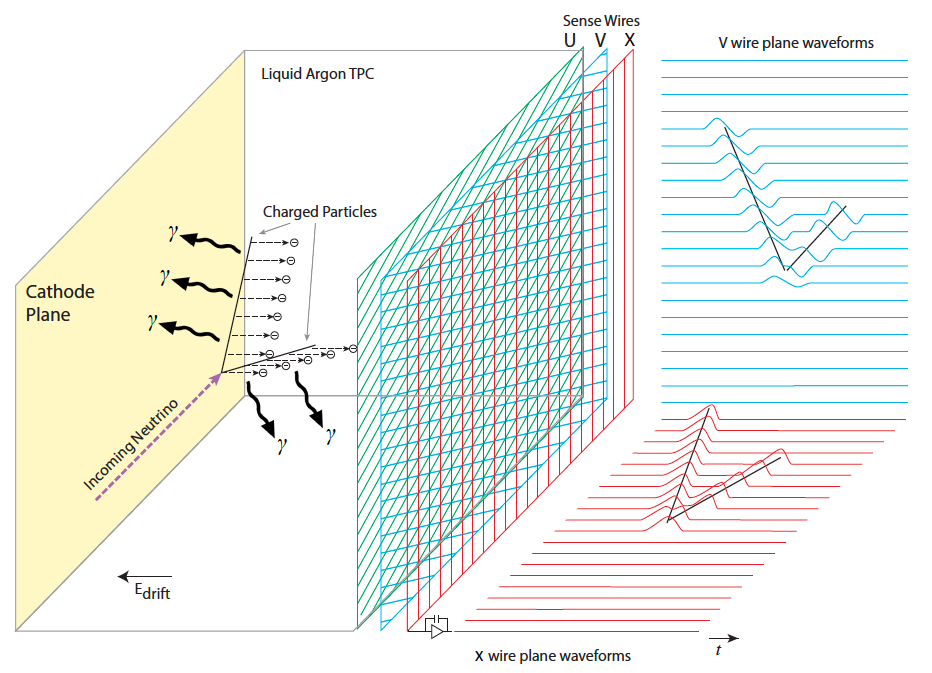
\includegraphics[width=0.75\textwidth]{TheBoPicture.png} 
\end{dunefigure}

\begin{dunefigure}[A \nominalmodsize DUNE far detector SP module]{fig:DUNESchematic1ch1}
{Schematic of a \nominalmodsize \dword{dune} \dword{fd} \dword{spmod}, showing the alternating anode (A) and cathode (C) planes that divide the \dword{lartpc} into four separate drift volumes. The red arrows point to one top and one bottom \dword{fc} module and to the rear endwall field cage.}
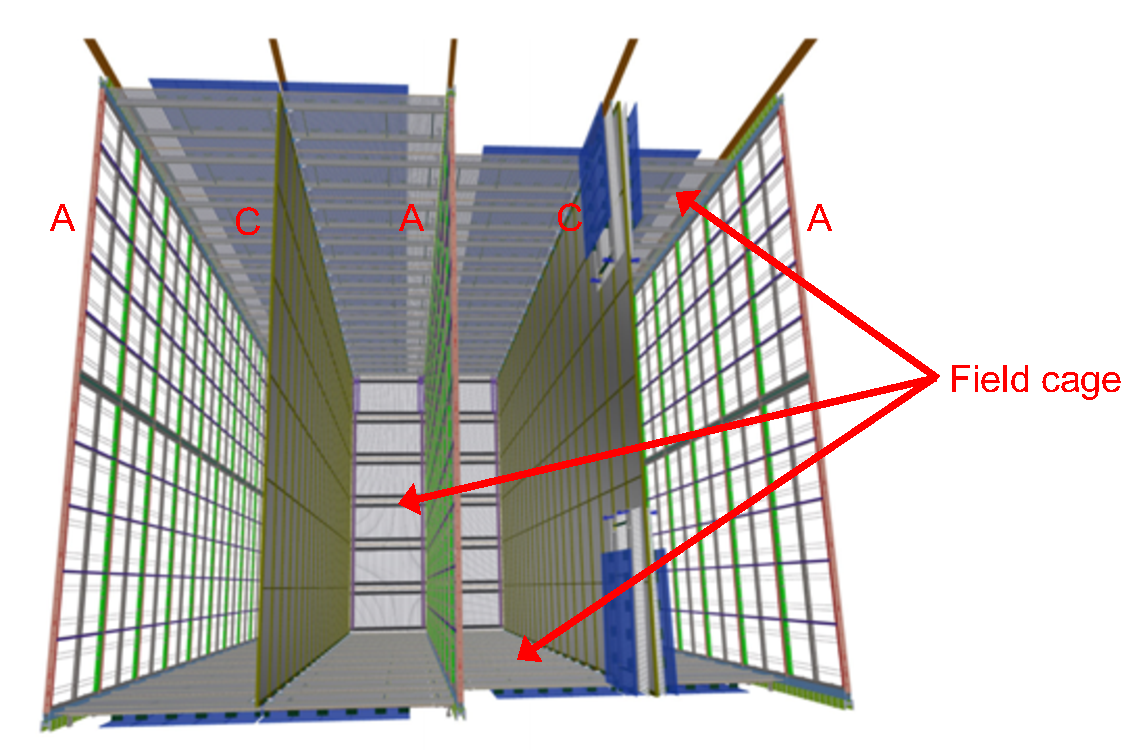
\includegraphics[width=0.65\textwidth]{DUNESchematic.pdf}
\end{dunefigure}

A \dword{spmod} is instrumented with three module-length anode planes constructed from \SI{6}{m} high by \SI{2.3}{m} wide \dword{apa}s, stacked two \dword{apa}s high and 25 wide, for 50 \dword{apa}s per plane, or 150 total. 
Each \dword{apa} is two-sided with three layers of active wires forming a grid on each side of the \dword{apa}.
 The relative voltage between the layers is chosen to ensure the transparency to the drifting electrons of the first two layers ($U$ and $V$). These layers produce bipolar induction signals as the electrons pass through them. The final layer ($X$) collects the drifting electrons, resulting in a unipolar signal. The pattern of ionization collected on the grid of anode wires provides the reconstruction in the remaining two coordinates perpendicular to the drift direction.


Scintillation photons are detected in 
novel \dword{pd} modules, based on  
a light-trap concept known as 
ARAPUCA~\cite{arapuca_jinst,arpkLNLS,Segreto:2018jdx} that   
utilizes dichroic filters, wavelength-shifting plates and 
\dword{sipm} read-out. The variant of this technology in 
the DUNE baseline design (X-ARAPUCA) is described in Volume~\volnumbersp{}.  
The \dword{pd} modules 
are placed in the inactive space between the 
innermost wire planes of the \dword{apa}s, installed through 
slots in a pre-wound \dword{apa} frame. 
There are ten \dword{pd} modules per \dword{apa} for a total of 
\num{1500} per \dword{spmod}.  Of these, \num{500} are mounted in 
central \dword{apa} frames and must collect light from both 
directions, 
and \num{1000} are mounted in frames  near the %vessel 
cryostat walls and collect light from only one direction. 

\FloatBarrier
%%%%%%%%%%%%%%%%%%%%%%%%%%%%%%%%%%%%%%%%
\subsection{Dual-phase Technology}
\label{sec:fddp-exec-splar}

The \dword{dp} operating principle, illustrated in Figure~\ref{fig:DPprinciplech1}, is very similar to that of the \dword{sp}. % design. 
 Charged particles that traverse the active volume of the \dword{lartpc} ionize the medium while also producing scintillation light.  The ionization electrons drift along an \efield towards a segmented anode where they deposit their charge. Scintillation light is measured in \dwords{pd} that view the volume from below. % and where  \dwords{pd} pick up the scintillation light. 
 
 
\begin{dunefigure}[The DP LArTPC operating principle]{fig:DPprinciplech1}{The general operating principle of the \dword{dp} \dword{lartpc}.}
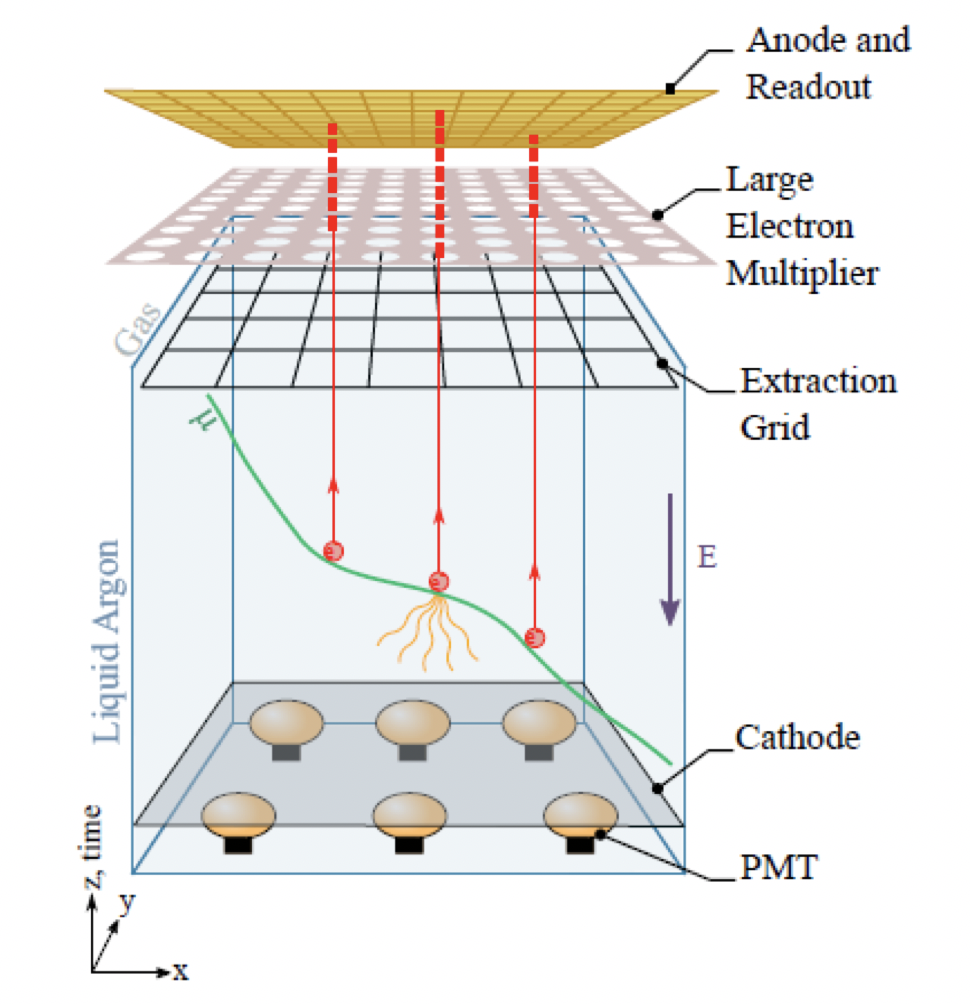
\includegraphics[width=0.5\textwidth]{dualphase-principle}
\end{dunefigure}

%The key differentiating concept of the \dword{dp} design is the amplification of the ionization signal in an avalanche process that takes place in a layer of argon gas above the \dword{lar}.  
In this design, shown in Figure~\ref{fig:DPdet1ch1}, electrons drift upward toward an extraction grid just below the liquid-vapor interface. 
After reaching the grid, an \efield stronger than the \dpnominaldriftfield{} drift field extracts the electrons from the liquid up into the gas phase. Once in the gas, electrons encounter micro-pattern gas detectors, called \dwords{lem}, with high-field regions. The \dwords{lem} amplify the electrons in avalanches that occur in these high-field regions. The amplified charge is then collected and recorded on a \twod anode
consisting of two sets of %\SI{3.125}{mm}-pitch 
gold-plated copper strips that provide the $x$ and $y$ coordinates (and thus two views) of an event. 

\begin{dunefigure}[A \nominalmodsize DUNE far detector DP module]{fig:DPdet1ch1}
  {Schematic of a \nominalmodsize \dword{dune} \dword{fd} \dword{dp} \dword{detmodule} with cathode, \dwords{pmt}, \dword{fc}, and anode plane with \dwords{sftchimney}. The drift direction is vertical in the case of a \dword{dpmod}.}
  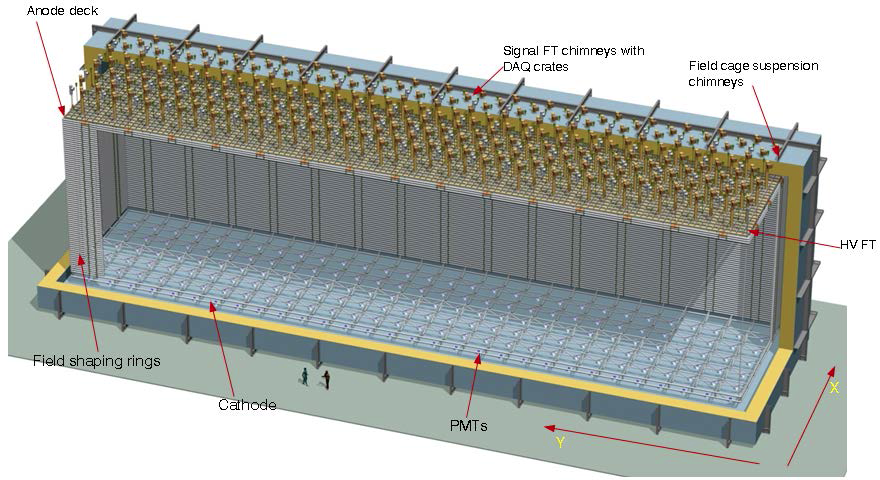
\includegraphics[width=0.9\textwidth]{DUNE-CDR-detectors-volume-optim.png}
\end{dunefigure}

 The extraction grid, \dword{lem}, and anode are assembled into three-layered sandwiches with precisely defined inter-stage distances and inter-alignment,  which are then connected horizontally into \num{9}~m$^2$ modular detection units. These detection units are called \dwords{crp}.

The precision tracking and calorimetry offered by the \dword{dp} technology provides excellent capabilities for identifying interactions of interest while mitigating sources of background.  Whereas the \dword{sp} design has multiple drift volumes, the \dword{dpmod} design allows a single, fully homogeneous \dword{lar} volume with a much longer drift length.

A simple array of \dwords{pmt} coated with a wavelength-shifting material is located below the cathode. The \dwords{pmt} record  the time and pulse characteristics of the incident light.



\FloatBarrier
%%%%%%%%%%%%%%%%%%%%%%%

\subsection{ProtoDUNEs: Far Detector Prototypes}

The \dword{dune} collaboration has constructed 
two large prototype detectors (\dwords{protodune}), \dword{pdsp} and \dword{pddp}, located at CERN. %one using \single readout (\dword{pdsp}) and the other \dual readout (\dword{pddp}).
 Each is approximately one-twentieth the size of a \dword{dune} \dword{detmodule} and uses components identical in size to those of the full-scale module. \dword{pdsp} has the same \spmaxdrift maximum drift length as the full \dword{spmod}. \dword{pddp} has a \SI{6}{m} maximum drift length, half that planned for the \dword{dpmod}. See the photos in Figures~\ref{fig:protodunes_northarea} and~\ref{fig:protodunes_interior}.

\begin{dunefigure}[ProtoDUNE cryostats at the CERN Neutrino Platform]
{fig:protodunes_northarea}
{ProtoDUNE-SP and ProtoDUNE-DP cryostats in the CERN Neutrino Platform in CERN's North Area.  The view is from the downstream end of the hall with respect to the beam lines.  At front and  center is the top of the \dword{pdsp} cryostat.  The \dword{pddp} cryostat with its painted red steel support frame visible is located at the rear of the photo on the right side of the hall.} 
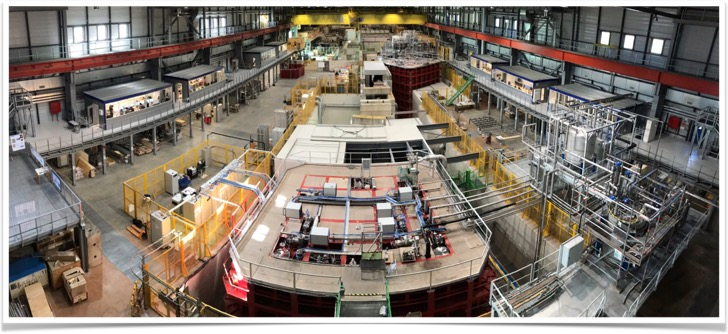
\includegraphics[width=0.9\linewidth]{neutrinoplatform.jpg}
\end{dunefigure}

\begin{dunefigure}[Interior views of the ProtoDUNEs]
{fig:protodunes_interior}
{Interior views of ProtoDUNE-SP (left) and ProtoDUNE-DP (right). For ProtoDUNE-SP, one of two identical drift volumes is shown.}
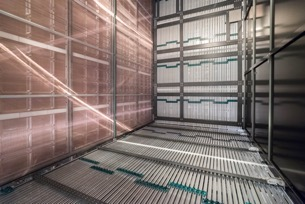
\includegraphics[width=0.46\linewidth]{graphics/ProtoDUNE-sp-interior.jpg}\hspace{0.05\linewidth}
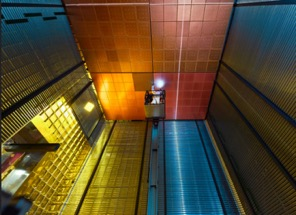
\includegraphics[width=0.44\linewidth]{graphics/protodune-dp-interior.jpg}
\end{dunefigure}

These large-scale prototypes allow us to validate key aspects of 
the \dword{tpc} designs, test engineering procedures, and collect 
valuable calibration data using a hadron test beam. 

The construction phase of \dword{pdsp} was finished in July 2018, 
and the detector was filled with \dword{lar} in August 2018. The 
detector collected hadron beam data and cosmic rays during the 
fall of 2018 and continues to collect cosmic-ray data.
The construction of the \dword{pddp} detector was completed in 
June of 2019, and started operations in September 2019.  

Data taken with the \dword{pdsp} detector demonstrates its 
excellent performance and has already provided valuable 
information on the design, calibration, and simulation of the 
\dword{dune} \dword{fd}. In all, $99.7\%$ of the 15360 \dword{tpc} 
electronics channels are responsive in the \dword{lar}. The 
%\dword{enc} 
equivalent noise charge
amounts to $\approx 550$ $e^{-}$ on the collection 
wires and $\approx 650$ $e^{-}$ on the induction wires. An average 
\dword{s/n} of 38 for the collection plane is measured using 
cosmic-ray muons, while for the two induction planes, the 
\dword{s/n} is 14 (U) and 17 (V), exceeding the requirement  
% of a ratio $9/1$ 
for the \dword{dune} \dword{fd}. 
The \dword{pdsp} photon detection system has also operated stably, 
demonstrating the principle of effective collection of 
scintillation light in a large-volume \dword{lartpc} with 
detectors embedded within the \dwords{apa}.


%%%%%%%%%%%%%%%%%%%%%%%%%%%%%%%%%%%%%%%%%%%%%%%%%%%%%%%%%%%%%%%%
% This section taken from Volume 1, section 1.4
\section{Near Detector Complex}
\label{sec:physics-nd-overview}

The \dword{dune} \dword{nd} is crucial for the success of the \dword{dune} physics program. It is used to precisely measure the neutrino beam flux and flavor composition. Comparing the measured neutrino energy spectra at the near and far site allows us to disentangle the different energy-dependent effects that modulate the beam spectrum and to reduce the systematic uncertainties to the level required for discovering \dword{cp} violation. In addition, the \dword{nd} will measure neutrino-argon interactions with high precision using both gaseous and liquid argon, which will further reduce the systematic uncertainties associated with the modeling of these interactions.


The \dword{nd} hall will be located \SI{574}{m} downstream from the target and will include three primary detector components, shown in Figure~\ref{fig:neardetectors}  and listed in Table~\ref{tab:NDsumm}. Two of them can move off beam axis, providing access to different neutrino energy spectra. The movement off axis, called \dword{duneprism}, provides a crucial extra degree of freedom for the \dword{nd} measurement and is an integral part of the \dword{dune} \dword{nd} concept. 


\begin{dunefigure}[DUNE near detector]
{fig:neardetectors}
{DUNE Near Detector. The beam enters from the right and encounters
the \dword{lartpc}, the MPD, and the SAND on-axis beam monitor.}
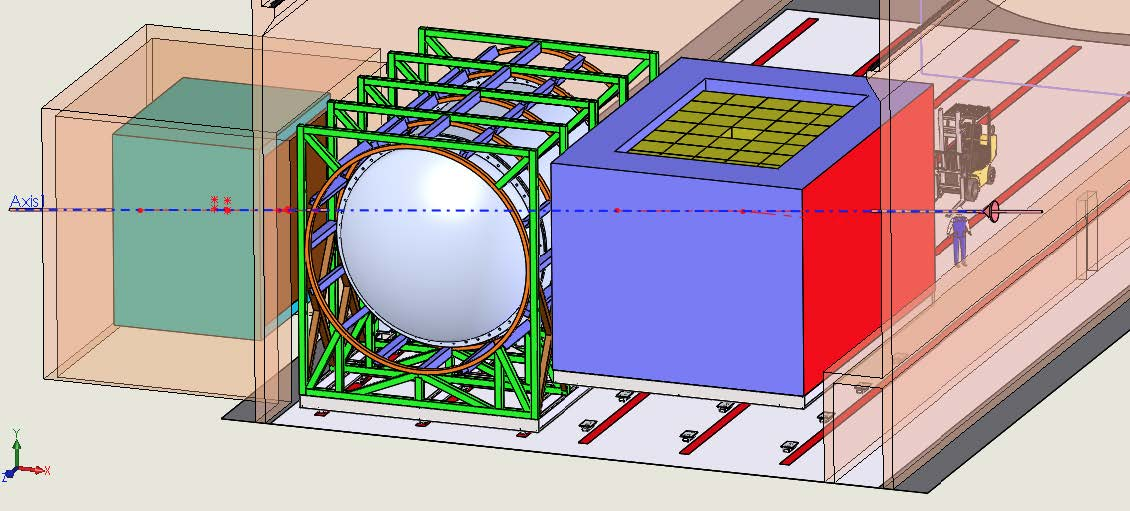
\includegraphics[width=0.9\textwidth]{ND_Detectors.jpg}
\end{dunefigure}

The three detector components -- a \dword{lartpc} called \dword{arcube}; a \dword{hpgtpc} within a magnet surrounded by an \dword{ecal}, together called \dword{mpd}; and an on-axis beam monitor called \dword{sand} -- serve important individual and overlapping functions in the mission of the \dword{nd}. 
The \dword{dune} \dword{nd} is shown schematically in the \dword{dune} \dword{nd} hall in Figure~\ref{fig:NDHallconfigs}.  
Table~\ref{tab:NDsumm} provides a high-level overview of the three components of the \dword{dune} \dword{nd} along with the off-axis capability.  

\begin{dunetable}[Components of the DUNE ND]
{p{.22\textwidth}p{.22\textwidth}p{.22\textwidth}p{.22\textwidth}}
{tab:NDsumm}{This table gives a high-level breakdown of the three major detector components and the capability of movement for the DUNE ND along with function and primary physics goals.}
Component & Essential Features  & Primary function & Select physics aims \\
 \toprowrule
LArTPC (ArgonCube) & Mass  & Experimental control for the Far Detector & $\numu$($\overline{\nu}_{\mu}$) CC \\
          & Target nucleus Ar &  Measure unoscillated $E_\nu$ spectra   & $\nu$-e$^{-}$ scattering   \\
          &  Technology FD-like    &  Flux determination  &  $\nue +$$\overline{\nu}_{e}$ CC  \\
          &  &  &  Interaction model \\ \colhline
Multipurpose detector (MPD) & Magnetic field & Experimental control for the LArTPCs & $\numu$($\overline{\nu}_{\mu}$) CC \\
  &  Target nucleus Ar & Momentum analyze liquid Ar $\mu$ & $\nue$ CC, $\overline{\nu}_{e}$ \\
  & Low density & Measure exclusive final states with low momentum threshold & Interaction model \\  \colhline
%
%\dword{3dsts} 
On-axis beam monitor \hfill (\dword{sand})
 & On-axis & Beam flux monitor &  On-axis flux stability \\ 
  & Mass & Neutrons & Interaction model \\ 
& Magnetic field &  & A dependence \\
    & CH target & & $\nu$-e$^{-}$ scattering \\ \colhline \colhline
    
    DUNE-PRISM (capability) & LArTPC$+$MPD move off-axis & Change flux spectrum &  Deconvolve xsec*flux \\ 
 & & & Energy response \\
 & & & Provide FD-like energy spectrum at ND\\ 
% & & & {\   }differences \\
 & & & ID mismodeling \\ \colhline
\end{dunetable}

The \dword{arcube} detector contains the same target nucleus and shares some aspects of form and functionality with the \dword{fd}. The differences are necessitated by the expected high intensity of the neutrino beam at the \dword{nd}.  This similarity in target nucleus and, to some extent, technology, reduces sensitivity to nuclear effects and detector-driven systematic uncertainties in extracting the oscillation signal at the  \dword{fd}. 
%Using the same target nucleus is particularly important because extrapolation of cross sections between nuclear targets with different atomic number is highly model-dependent. 
The \dword{arcube} \dword{lartpc} is large enough to provide high statistics ($\num{1e8} {\numu \text{ charged current events/year on axis}}$), and its volume is sufficiently large to provide good hadron containment.  The tracking and energy resolution, combined with the mass of the \dword{lartpc}, will allow measurement of the flux in the beam using several techniques, including the rare process of $\nu$-e$^{-}$ scattering.

\begin{dunefigure}[DUNE ND Hall with component detectors]
{fig:NDHallconfigs}
{\dword{dune} \dword{nd} hall shown with component detectors all in the on-axis configuration (left) and with the \dword{lartpc} and \dword{mpd} in an off-axis configuration (right). The on-axis monitor \dword{sand} is shown in position on the beam axis. 
%The beam axis is shown.  The beam enters the hall at %the bottom of the drawings moving from right to left.
}
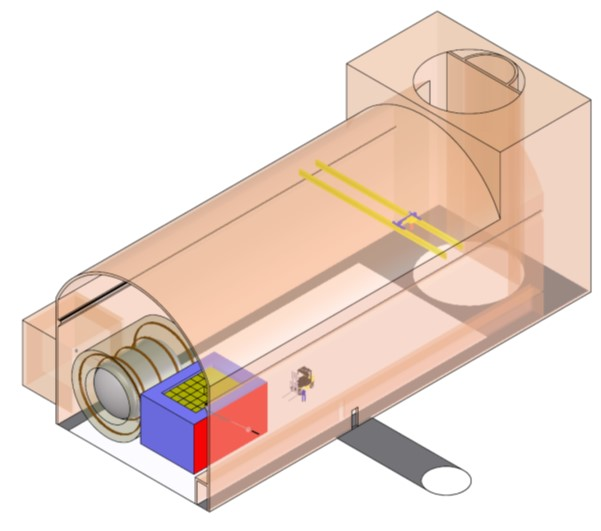
\includegraphics[width=0.49\textwidth]{graphics/NDHall_onaxis.jpg}
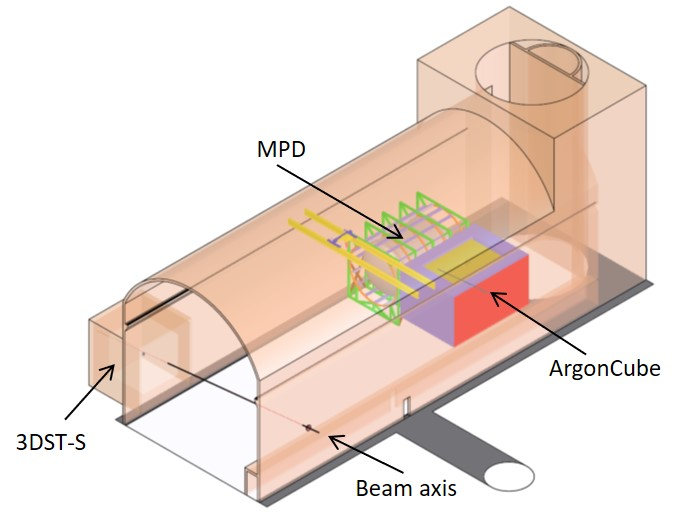
\includegraphics[width=0.49\textwidth]{graphics/NDHall_offaxis.jpg}
\end{dunefigure}

The \dword{lartpc} begins to lose acceptance for muons with a measured momentum higher than 
$\approx$0.7~GeV/c because the muons will not be contained in the \dword{lartpc} volume.  Because the muon momentum is a critical component of determining the neutrino energy, a magnetic spectrometer is needed downstream of the \dword{lartpc} to measure the charge sign and momentum of the muons.  In the \dword{dune} \dword{nd} concept, this function is accomplished by the \dword{mpd}, which consists of a \dword{hpgtpc} surrounded by an \dword{ecal} in a \SI{0.5}{T} magnetic field. The \dword{hpgtpc} provides a lower density medium with excellent tracking resolution for the muons from the \dword{lartpc}.  

In addition, neutrinos interacting with the argon in the gas \dword{tpc} constitute a sample of $\nu$-argon events that can be studied with a very low charged-particle tracking threshold and excellent resolution superior to \dword{lar}. The high pressure yields a sample of $\num{2e6}{\numu \text{-CC events/year}}$ for these studies. These events will be valuable for studying the charged particle activity near the interaction vertex because this detector can access lower momenta protons than the \dword{lar} detector and can better identify charged pions.  The lack of secondary interactions in these samples will be helpful for identifying the particles produced in the primary interaction and modeling secondary interactions in denser detectors.
%which are known to be important \cite{Friedland:2018vry}.

The \dword{ecal} adds neutral particle (mainly $\gamma$'s and 
neutrons) detection capability otherwise lacking in the \dword{mpd}.
NC-$\pi^0$ backgrounds to $\nu_e$ CC interactions can be studied, 
for example.  
Additionally, neutron production in neutrino-nucleus interactions 
is poorly understood: the presence of the \dword{ecal} 
opens the possibility of identifying neutrons via time-of-flight.

The \dword{lartpc} and \dword{mpd} can be moved sideways up to 33 m to take data in positions off the beam axis.  This capability is referred to as \dword{duneprism}. As the detectors move off-axis, the incident neutrino flux spectrum changes, with the mean energy dropping and the spectrum becoming more monochromatic.  Though the neutrino interaction rate drops off-axis, the intensity of the beam and the size of the \dword{lartpc}  combine to yield ample statistics even in the off-axis positions.
The \dword{dune} concept is based on reconstructing the energy-dependent neutrino spectrum and
comparing the far and near sites. The ability to modify the energy spectrum at the near site by measuring at the off-axis locations will allow disentangling otherwise degenerate effects due to systematic biases of the energy reconstruction.

The final component of the \dword{dune} \dword{nd} suite (\dword{sand}) is the on-axis beam monitor that remains in fixed position at all times and serves as a dedicated neutrino spectrum monitor. 
It can also provide an excellent on-axis neutrino flux determination that can be used as an important point of comparison and a systematic crosscheck for the flux as determined by \dword{arcube}.

%%%%%%%%%%%%%%%%%%%%%%%%%%%%%%%%%%%%%%%%%%%%%%%%%%%%%%%%%%%%%%

